% Copyright 2020-2023 Robert Bosch GmbH

% Licensed under the Apache License, Version 2.0 (the "License");
% you may not use this file except in compliance with the License.
% You may obtain a copy of the License at

% http://www.apache.org/licenses/LICENSE-2.0

% Unless required by applicable law or agreed to in writing, software
% distributed under the License is distributed on an "AS IS" BASIS,
% WITHOUT WARRANTIES OR CONDITIONS OF ANY KIND, either express or implied.
% See the License for the specific language governing permissions and
% limitations under the License.

\hypertarget{tool-features}{%
\section{Tool features}\label{tool-features}}

The \pkg\ facilitates seamless integration and synchronization between multiple
issue tracking platforms. The main operations include:

\begin{enumerate}
   \item Configuration Parsing
         \begin{itemize}
            \item Reads the JSON configuration file to understand the
                  synchronization scope and behavior.
         \end{itemize}

   \item Issue Collection
         \begin{itemize}
            \item Fetches issues from GitHub, Gitlab and Jira based on the
                  specified conditions.
            \item Uses user mappings to ensure issues are associated correctly
                  across platforms.
         \end{itemize}

   \item Issue Update
         \begin{itemize}
            \item Updates the source issues with RTC IDs and planning data after
                  synchronization.
         \end{itemize}

   \item Synchronization to RTC
         \begin{itemize}
            \item Creates or updates work items in RTC with the collected issues.
            \item Includes planning data provided by RTC.
         \end{itemize}
\end{enumerate}

The tool also provides additional features to enhance the synchronization process,
please refer \hyperlink{additional-features}{Additional features} section for more details.

\hypertarget{tool-usage}{%
\section{Tool usage}\label{tool-usage}}

Use below command to get tools's usage:

\begin{pythonlog}
IssueSyncTool -h
\end{pythonlog}

The tool's usage should be showed as below:

\begin{pythonlog}
usage: IssueSyncTool (Tickets Sync Tool) [-h] --config CONFIG [--dryrun] [--csv] [-v]

IssueSyncTool sync ticket|issue|workitem between tracking systems such as Github Issue, JIRA and IBM RTC

optional arguments:
  -h, --help       show this help message and exit
  --config CONFIG  path to configuration json file
  --dryrun         if set, then just dump the tickets without syncing
  --csv            if set, then store the sync status to csv file sync_status.csv
  --nosync         If set, issues with the 'nosync' label will not be synced,
                   and any previously synced issues with this label will be closed.
  --status-only    If set, only update status of synced issue on destination tracker.
  -v, --version    version of the IssueSyncTool
\end{pythonlog}

Sample command to run \pkg\ with the configuration JSON file and save sync
status as csv file:

\begin{pythonlog}
IssueSyncTool --config <your-config-file> --csv
\end{pythonlog}

\hypertarget{config-file}{%
\section{JSON Configuration File}\label{config-file}}

The tool uses a JSON configuration file to define synchronization behavior.
Below is an explanation of the sample configuration:

\subsection{Source and Destination Platforms}
\begin{pythoncode}
{
   "source": ["github", "gitlab", "jira"],
   "destination": ["rtc"]
   ...
}
\end{pythoncode}
This configuration specifies GitHub and Jira as sources and RTC as the
destination for synchronization.

\subsection{Tracker Configurations}
\begin{pythoncode}
{
   ...
   "tracker": {
      "github": {
         "project" : "test-fullautomation",
         "token": "<your-PAT>",
         "repository": [
            "python-jsonpreprocessor"
         ],
         "condition": {
            "state": "open",
            "exclude": {
               "assignee": "empty",
               "labels": "0.13.1"
            }
         }
      },
      ...
   }
   ...
}
\end{pythoncode}

Above code is sample configuration of Github tracker which contain the
information about:

\begin{itemize}
    \item \textbf{Project:} Github project \pcode{"test-fullautomation"}
    \item \textbf{Token:} A personal access token for authentication.
    \item \textbf{Repositories:} List of repositories to collect issues from.
    \item \textbf{Condition:} Define the condition (query) to collect the issues.
          \begin{itemize}
            \item \pcode{"state"}: Syncs only issues in the specified state,
                  e.g., \pcode{"open"}.
            \item \pcode{"exclude"}: Specifies negative conditions. For example:
            \begin{itemize}
               \item \pcode{"assignee": "empty"}: Excludes issues with no assignee.
               \item \pcode{"labels": "0.13.1"}: Excludes issues labeled \pcode{"0.13.1"}.
            \end{itemize}
          \end{itemize}
\end{itemize}

The other tracker can be configured as the same way.

\subsection{User Mapping}
User mapping ensures that the correct user is assigned in the synchronization
process across different platforms.
In the configuration file, each user is mapped to their corresponding accounts
across GitHub, Jira, Gitlab and RTC. This mapping helps to ensure that the right
assignee is applied to issues in the appropriate tracker system.

\begin{itemize}
   \item The \texttt{user} section of the configuration file specifies the
         mapping between the users' names in GitHub, Gitlab, Jira and RTC.
   \item This ensures that the correct user is set as the assignee in each
         platform when syncing issues.
   \item For instance, when syncing an issue from Jira to RTC, the tool will
         automatically assign the same user (as per the mapping) to the issue in RTC.
   \item If the user has different usernames across platforms
         (e.g., "githubUser" in GitHub, "jiraUser" in Jira, and "rtcUser" in RTC),
         the tool ensures the correct mapping is applied so that all systems
         reflect the same assignee.
\end{itemize}

Example configuration:
\begin{pythoncode}
{
   ...
   "user": [
      {
         "name": "Tran Duy Ngoan",
         "github": "ngoan1608",
         "jira": "ntd1hc",
         "gitlab": "ntd1hc",
         "rtc": "ntd1hc"
      },
      ...
   ]
}
\end{pythoncode}

In this example:
\begin{itemize}
    \item The user \plog{Tran Duy Ngoan} is mapped to \plog{ngoan1608} in
          GitHub, \plog{ntd1hc} in Jira, and \plog{ntd1hc} in RTC.
    \item When syncing issues between GitHub, Jira, and RTC, the tool ensures
          that issues assigned to \plog{ngoan1608} in GitHub and
          \plog{ntd1hc} in Jira will be assigned to \plog{ntd1hc} in RTC,
          ensuring consistent user data across all platforms.
\end{itemize}

\subsection{Component Mapping}
This configuration allows issues from specific repositories (components) to be
synchronized to a destination tracker with a short name prefix in the issue
title.
This helps standardize and identify issues based on their originating repository
in the destination tracker.

Example configuration:
\begin{pythoncode}
{
   ...
   "component_mapping": {
      "python-genpackagedoc": "GenPkgDoc",
      "python-extensions-collection": "PyExtColl",
      "python-jsonpreprocessor": "JPP",
      "python-testresultdbaccess": "WebApp",
      ...
   }
   ...
}
\end{pythoncode}

Key-Value Explanation:
\begin{itemize}
   \item Key: The name of the repository/component from which the issue
         originates (e.g., \plog{python-genpackagedoc}).
   \item Value: The short name that will be used as a prefix in the issue title
         when synchronized to the destination tracker (e.g., \plog{GenPkgDoc}).
\end{itemize}

When an issue is synchronized from a source repository to the destination
tracker, the feature automatically applies the following changes:
\begin{itemize}
   \item Looks up the repository name in the \pcode{component_mapping} configuration.
   \item Prepends the corresponding short name to the issue title as a prefix.
\end{itemize}

Example issue:
\begin{itemize}
   \item Repository: \plog{python-genpackagedoc}
   \item Original Issue Title: \plog{Fix missing documentation}
   \item Destination Tracker Issue Title: \plog{[GenPkgDoc] Fix missing documentation}
\end{itemize}

\subsection{Sprint-Version Mapping Configuration}

Consider a team delivering both \pcode{AIO} and \pcode{DevAtServ} in the same
sprint cycle.
Each product has its own development timeline and release schedule.

This configuration allows SyncTool to determine and synchronize the correct
version label on the original issue, based on the sprint information found in
the destination issue.

The \pcode{sprint_version_mapping} configuration defines the mapping between
sprint identifiers and the specific versions of multiple software components
(or products) being developed and released in parallel.
\begin{itemize}
  \item Each key in the mapping (e.g., \pcode{PI25.2.1}, \pcode{PI25.3.1})
        represents a sprint or planning increment (PI).
  \item Each value is a nested mapping of product names (e.g., \pcode{AIO},
        \pcode{DevAtServ}) to their respective release version numbers.
\end{itemize}

Example Configuration:
\begin{pythoncode}
{
   ...
   "sprint_version_mapping": {
      "PI25.2.1" : {
         "AIO" : "0.14.0",
         "DevAtServ" : "0.1.0"
      },
      "PI25.2.2" : {
         "AIO" : "0.14.1",
         "DevAtServ" : "0.1.0"
      },
      "PI25.2.4" : {
         "AIO" : "0.14.1",
         "DevAtServ" : "0.1.0"
      },
      "PI25.3.1" : {
         "AIO" : "0.14.2",
         "DevAtServ" : "0.1.0"
      }
   }
}
\end{pythoncode}

This configuration plays a critical role in environments where teams are:
\begin{itemize}
  \item Developing \textbf{multiple software products} in parallel
        (e.g., \pcode{AIO}, \pcode{DevAtServ}).
  \item Practicing Agile or SAFe methodologies with iterative sprint-based
        planning.
\end{itemize}

\hypertarget{additional-features}{%
\section{Additional features}\label{additional-features}}

\subsection{\pcode{nosync} Label}
The \pcode{nosync} label is a special label that can be applied to issues in the
source tracker (e.g., GitHub, Jira, Gitlab) to prevent them from being synced to
the destination tracker (RTC).

When the \pcode{nosync} label is applied to an issue, the tool will not sync that
issue to RTC.

If an issue was previously synced and later labeled with \pcode{nosync}, the tool
will close the issue in RTC to indicate that it should no longer be tracked.

To use this feature, add the \pcode{--nosync} argument when running the tool:

\begin{pythonlog}
IssueSyncTool --config <your-config-file> --nosync
\end{pythonlog}

\subsection{Status-only Update}
The \pcode{--status-only} argument allows you to update only the status of
previously synced issues on the destination tracker (RTC).

This feature is useful when you want to update the status of issues without
modifying other fields or creating new work items.

To use this feature, add the \pcode{--status-only} argument when running the tool:

\begin{pythonlog}
IssueSyncTool --config <your-config-file> --status-only
\end{pythonlog}

\newpage
\subsection{User-defined Workflow (only for RTC destination tracker)}
The tool supports user-defined workflows (state transitions) in RTC.

You can configure the tool to update the status of issues based on the workflow
defined in RTC.

At least, all actions from \plog{New} to \plog{Done} and vice-versa should be
defined in this configuration to ensure the tool can update the status of issues
correctly.

Example of user-defined workflow in RTC:

\begin{figure}[h!]
   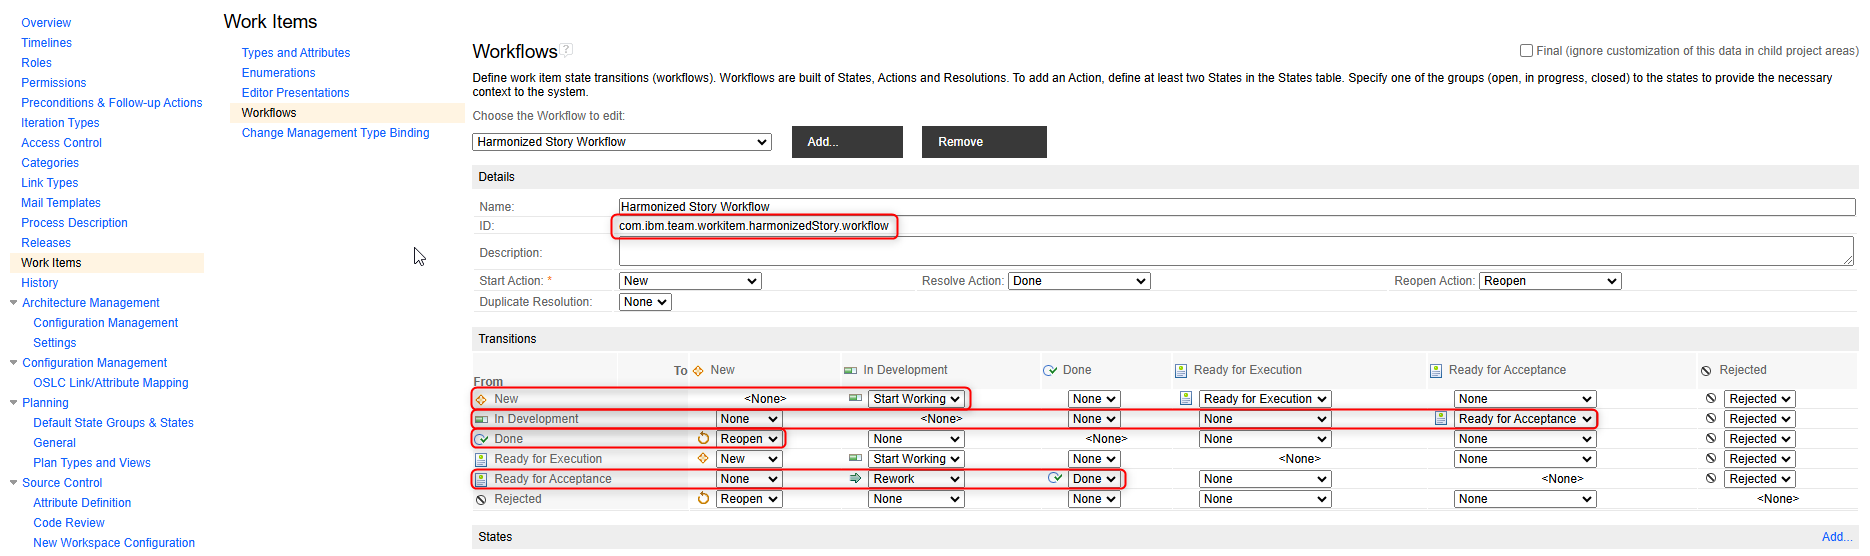
\includegraphics[width=1\linewidth]{./pictures/user-defined-workflow.png}
   \caption{User-defined workflow in RTC}
\end{figure}

To use this feature, add the following configuration to the JSON file:

\begin{pythoncode}
{
   ...
   "rtc": {
      ...
      "workflow_id" : "com.ibm.team.workitem.harmonizedStory.workflow",
      "state_transition": {
         "Start Working": [ "New", "In Development"],
         "Ready for Acceptance": ["In Development", "Ready for Acceptance"],
         "Done": ["Ready for Acceptance", "Done"],
         "Reopen": ["Done", "New"]
      }
   }
   ...
}
\end{pythoncode}

In this example:
\begin{itemize}
   \item The \pcode{state_transitions} section defines the allowed state
         transitions for issues in RTC.
   \item For instance, an issue in the \pcode{open} state can transition to
         \pcode{in progress}, and so on.
   \item By defining the state transitions, you can ensure that issues are
         updated according to the workflow defined in RTC.
\end{itemize}

\subsection{csv Output}
The \pcode{--csv} argument allows you to store the sync status of issues in a
CSV file named \pcode{sync_status.csv}.

This file contains information about the sync process, including the issue ID,
source tracker, destination tracker, and sync status.

To use this feature, add the \pcode{--csv} argument when running the tool:

\begin{pythonlog}
IssueSyncTool --config <your-config-file> --csv
\end{pythonlog}

Sample output in \pcode{sync_status.csv}:
\begin{pythonlog}
No., Ticket, Source Link, Destination ID, Stage
1, Github 2, https://github.com/ngoan1608/ntd1hc-sample-deb/issues/2, rtc , skipped
2, Github 1, https://github.com/ngoan1608/ntd1hc-sample-deb/issues/1, rtc 620036, synced

\end{pythonlog}

Possible value of status and their meaning:
\begin{itemize}
   \item \pcode{new}: The issue is new creation in the destination tracker.
   \item \pcode{synced}: The issue has been successfully synced to the
                         destination tracker.
   \item \pcode{not found}: The issue contains synced ID in title but was not
                            found in the destination tracker.
   \item \pcode{skipped}: The issue was not existing in destination tracker and
                          skipped during the sync process (when using
                          \plog{--status-only}).
   \item \pcode{nosync}: The issue has been labeled with \pcode{nosync} and will
                         not be synced to the destination tracker (when using
                         \plog{--nosync}).
   \item \pcode{closed nosync}: The issue was previously synced and later labeled
                                with \pcode{nosync}, so it has been closed in the
                                destination tracker (when using \plog{--nosync}).
\end{itemize}

\subsection{Default (Configurable) Values for New RTC Work Items}
When creating new work items in RTC, the tool allows you to define default
values for specific fields.
These values can be configured in the JSON configuration file under the
\pcode{rtc} section.

Example configuration:
\begin{pythoncode}
{
   ...
   "rtc": {
      ...
      "file_against": "RF-AIO",
      "planned_for": "Backlog_RFAIO",
      "project_scope": "Roadmap",
      ...
   }
   ...
}
\end{pythoncode}

Explanation of fields:
\begin{itemize}
   \item \pcode{file_against:} Sets the default \textbf{Filed Against}.
   \item \pcode{planned_for:} Sets the default \textbf{Planned For}.
   \item \pcode{project_scope:} Specifies the default \textbf{Project Scope} for
         new work items.
\end{itemize}

These default values ensure that newly created work items in RTC have consistent
and predefined attributes, reducing manual effort and ensuring alignment with
organizational standards.

\newpage

\hypertarget{attr-mapping}{%
\section{Sync Data and Attributes Mapping}\label{attr-mapping}}

\subsection{Sync Data: Attributes}

\begin{longtable}{|l|l|l|l|}
   \hline
   \textbf{Stage} & \textbf{Original tracker} & \textbf{Direction} & \textbf{Destination tracker}\\
   \hline
   \endfirsthead

   \hline
   \textbf{Stage} & \textbf{Original tracker} & \textbf{Direction} & \textbf{Destination tracker}\\
   \hline
   \endhead

   \multirow{8}{*}{\textbf{New}}
      & Component + Title & $\rightarrow$ & Title \\
      \cline{2-4}
      & URL + Description & $\rightarrow$ & Description \\
      \cline{2-4}
      & Assignee & $\rightarrow$ & Assignee \\
      \cline{2-4}
      & Priority & $\rightarrow$ & Priority \\
      \cline{2-4}
      & Story point & $\rightarrow$ & Story point \\
      \cline{2-4}
      & Labels & $\rightarrow$ & Labels \\
      \cline{2-4}
      & Relationship & $\rightarrow$ & Relationship \\
      \cline{2-4}
      & Title (e.g [xxx] Title) & $\leftarrow$ & ID \\
   \hline
   \multirow{12}{*}{\textbf{Sync}}
      & Component + Title & $\rightarrow$ & Title \\
      \cline{2-4}
      & URL + Description & $\rightarrow$ & Description \\
      \cline{2-4}
      & Relationship & $\rightarrow$ & Relationship \\
      \cline{2-4}
      & Labels & $\rightarrow$ & Labels \\
      \cline{2-4}
      & Sprint & $\leftarrow$ & Sprint \\
      \cline{2-4}
      & Version & $\leftarrow$ & Version \\
      \cline{2-4}
      & \multirow{2}{*}{Assignee}
         & $\leftarrow$ & Assignee (if set on Destination) \\
         \cline{3-4}
         & & $\rightarrow$ & Assignee (if not set on Destination) \\
      \cline{2-4}
      & \multirow{2}{*}{Story point}
         & $\leftarrow$ & Story point (if set on Destination) \\
         \cline{3-4}
         & & $\rightarrow$ & Story point (if not set on Destination) \\
      \cline{2-4}
      & \multirow{2}{*}{Priority}
         & $\leftarrow$ & Priority (is set on Destination) \\
         \cline{3-4}
         & & $\rightarrow$ & Priority (if not set on Destination) \\
   \hline
\end{longtable}


\subsection{Attributes Mapping on Trackers}

\begin{longtable}{|l|l|l|l|l|}
   \hline
   \textbf{Name} & \textbf{Github} & \textbf{Gitlab} & \textbf{JIRA} & \textbf{RTC} \\
   \hline
   \endfirsthead

   \hline
   \textbf{Name} & \textbf{Github} & \textbf{Gitlab} & \textbf{JIRA} & \textbf{RTC} \\
   \hline
   \endhead

   Title & Title & Title & Title & Title \\
   \hline
   URL & URL & URL & URL & URL \\
   \hline
   Assignee & Assignee & Assignee & Assignee & Owner \\
   \hline
   Component & Repository & Repository & Component & Component \\
   \hline
   Status & Labels & Labels & Status & Status \\
   & ("in work", "ready for verifying") & ("in work", "ready for verifying") & & \\
   \hline
   Story point & Labels (x pts) & Labels (x pts) & Estimate & Story point \\
   \hline
   Priority & Labels (prio x) & Labels (prio x) & Priority & Priority \\
   \hline
   Sprint & Labels (PI.*) & Labels (PI.*) & Sprint & Planned For \\
   \hline
\end{longtable}